\subsection{2D conservative transport in heterogeneous media}
\label{l_s_benchmark_2d_het}

In this benchmark conservative mass transport in a two-dimensional heterogeneous aquifer is tested. A secondary purpose of this benchmark is to test the functionality of assigning heterogeneous distributions of hydraulic conductivity and/or porosity. Furthermore, the functionality of reading in initial variable distributions from restart files is tested.

The 2D model aquifer has dimensions of 100 m by 100 m in x and y directions. The domain is uniformly discretized into 10000 quadrilateral elements with a constant x and y dimension of 1 m.

A randomly distributed but spatially correlated isotropic hydraulic conductivity field ($K_{eff} = 6.339\cdot10^{-4}$ ms$^{-1}$, $\sigma^2_{ln(K)}=1.0$) is provided, which is read in from a text file. Also porosity $n$ is not uniform. In the upper half of the aquifer (i.e. for $y > 50$ m) $n=0.5$, while in the lower half (i.e. for $y \leq 50$ m) $n=0.25$. A constant head boundary condition on the left hand side with a piezometric height of 10 m and a constant source term on the right hand side of the model with $q = -1.0$ md$^{-1}$ produce a steady state flow field. The steady state head distriburion is given as initial condition via a restart file. Longitudinal dispersivity has a value of 0.5, transversal dispersivity a value of 0.05 m. A conservative tracer is injected with a relative concentration value of 1.0 from two sources on the left hand side model boundary between $21.0 < y < 29.0 m$ and $71.0 < y < 79.0 m$, while the initial concentration of the tracer is zero all over the aquifer domain. The tracer diffusion coefficient is 1.0$\cdot10^{-9}$ m$^2$s$^{-1}$. A total simulation time of 25 days divided into 100 time steps is regarded.

\subsubsection*{Evaluation method}

Model results are compared to those of a previous GeoSys version.

\subsubsection*{Results}

Fig.~\ref{hetK_N_RFR} shows results of the flow and transport simulation after 25 days. Due to the higher porosity in the upper half of the aquifer, the tracer plume here migrates slower than in the lower half of the aquifer. Accordingly, tracer breakthrough curves measured 20 m downgradient of each source show a later breakthrough of the tracer from the upper source (green curve). In the right hand side plots of Fig.~\ref{hetK_N_RFR}, head distribution at the beginning and at the end of the simulation are plotted, demonstrating the correct reading in of data from a restart file.


\begin{figure}[htbp]
\centering
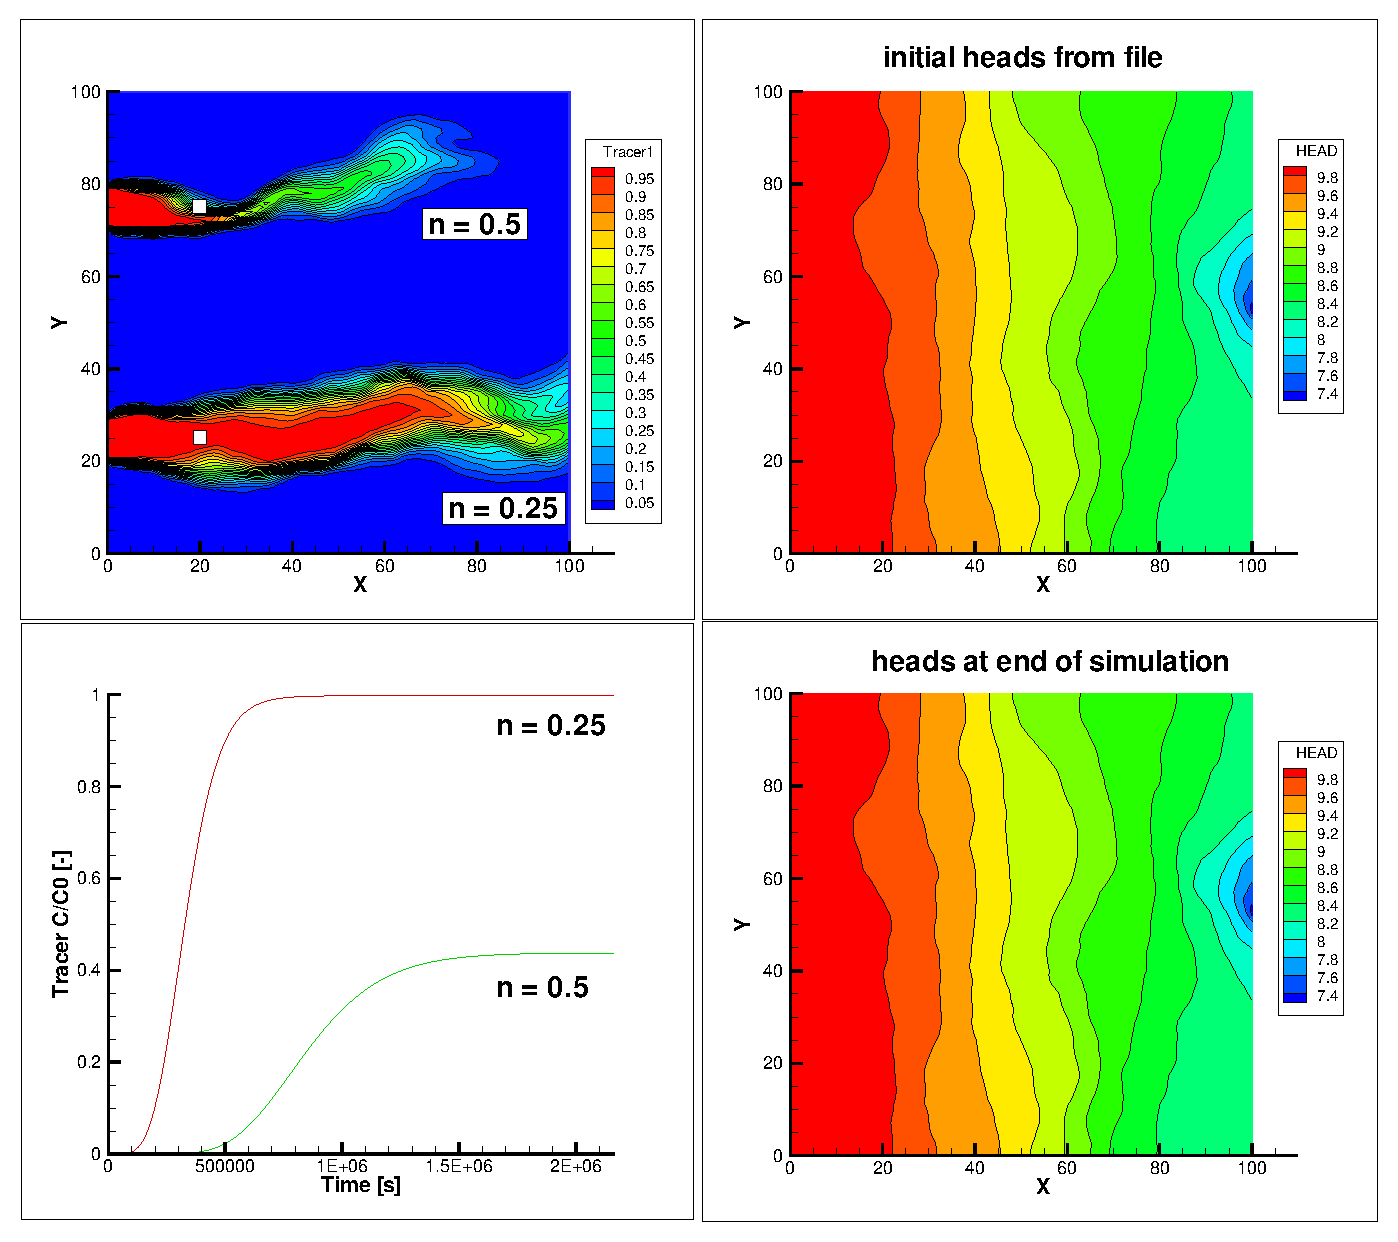
\includegraphics[width=0.8\textwidth]{C/figures/2d_hetKNRFR.eps}
\caption{Tracer plumes and breakthrough curves 20 m downgradient from both sources (left upper and lower diagram); Initial and final head distribution (right upper and lower diagram).}
\label{hetK_N_RFR}
\end{figure}



\begin{table}[htbp]
\centering
\begin{tabular}{|l|l|l|}
\hline
Benchmark & Type & Path \\
\hline
\texttt{2d\_hetk+n+restart}& HC &  benchmarks$\backslash$C$\backslash$hetk+n+restart  \\			
\hline
\end{tabular}
\end{table}
